\newpage
\chapter{Evaluating backgrounds in a dark matter search from a CMS Physics Analysis Summary (17/11/2016)}

So that I can begin doing some proper analysis, I will be using a CMS Physics Analysis Summary (PAS) \cite{CMS:2016pod} as a template. The information in the paper will be used to create an analysis file to run in \madanalysis. The paper states that 90\% of the backgrounds in this type of dark matter search can be attributed to Standard Model decays into $W^{\pm} / Z$ + jet. So I've created an input file for \madanalysis to apply the cuts given for the monojet analysis in the paper: $|\eta| < 2.5$, leading jet $p_{\mathrm{T}} > 100$ GeV, $\etmiss > 200$ GeV, no leptons, no $b$-quarks. This way I can plot the backgrounds that I generated previously for $pp \rightarrow W +$ jets and $pp \rightarrow Z +$ jets (with some minor changes: removing the lepton $p_{\mathrm{T}}$ cut, and generating more events). Then we get an estimate of these backgrounds for the DM search -- which will be enhanced with more events, etc., in the future -- and can then start thinking about implementing the other backgrounds for this search. Then we can look for a signal. At the LHC, monojets are used most prominently to look for dark matter particles. This because when the protons collide and produce dark matter, the incoming protons can emit gluons or jets before the collision and recoil from the dark matter, so you get a boosted jet because the DM particles are heavy.

The only problem, at the moment, with generating my backgrounds is the weight assigned to each event. The paper uses 12.9 fb$^{-1}$ of data, corresponding to a lot of events. With the \madgraph output that I've generated, I only ran 200,000 events for each process, corresponding to a luminosity $\mathcal{O}$(10 pb) [where the symbol $\mathcal{O}$ means "of order"]. So when I scale the luminosity in the \madanalysis input file to 12.9 fb$^{-1}$, it effectively scales the weight of each event by a certain amount to match that luminosity. With reliable data the weight of each event is $\sim$1, so the backgrounds I have generated at the time of writing are not suitable for detailed analysis. Obviously this will be rectified in the future, but for now I am just demonstrating the technique and the motivation behind the use of \madanalysis and these data.

The input and output files are displayed below. The values I have after the cuts can be compared with those from the paper via the link \url{http://cms-results.web.cern.ch/cms-results/public-results/preliminary-results/EXO-16-037/} under the "Additional Tables" heading. If I want to examine the .root file generated for each process that I'm importing, it is located in the path \textbf{$<$name of output folder$>$/Output/\_$<$label given to imported file$>$/TheMouth.root}.

The input file \textbf{DMbkgmonoj.ma}:

\lstinputlisting[language=Python, label={listing:dmmonojinput}, caption={The input file to analyse the monojet backgrounds for the dark matter search in \cite{CMS:2016pod}. File name: DMbkgmonoj.ma (v1).}]{./sec15/DMbkgmonojv1.ma}

Then I created some C++ macros to analyse the file \textbf{TheMouth.root} so that I could get the $y$-values of each bin in the \etmiss histogram and compare them with those from the paper. Because the entries in each bin must be multiplied by its weight -- given in the main.pdf file created during the \madanalysis run, which is fine because I need to run \madanalysis to generate the PDF and ROOT files before running the macros -- I've included that value as a \texttt{const double} in the global header \textbf{MouthGlobal.h}. In the same file, I've added a \texttt{TString} that contains the directory to \textbf{TheMouth.root}. So if I have several background files, as in this case, I can just modify the string once and it will apply globally (as I only need one source file and one header file to analyse \emph{any} \textbf{TheMouth.root} file). The commands are the same as with normal .root files; just open ROOT and type \verb!.x execMouth.C!.

The "daddy" macro \textbf{execMouth.C}:

\lstinputlisting[language=C++, caption={The "daddy" macro used to analyse TheMouth.root. File name: execMouth.C (v1).}]{./sec15/execMouthv1.C}

The global header file \textbf{MouthGlobal.h}:

\lstinputlisting[language=C++, label={listing:mouthglobalv1}, caption={The global header file to include when analysing TheMouth.root. File name: MouthGlobal.h (v1).}]{./sec15/MouthGlobalv1.h}

The source file \textbf{TheMouth.C}:

\lstinputlisting[language=C++, caption={The source file used to analyse TheMouth.root. File name: TheMouth.C (v1).}]{./sec15/TheMouthv1.C}

In the header file \textbf{TheMouth.h}, I've only included a few lines (the ones that need changing from their default when generated by ROOT). Some of the default "include" headers were also removed as they caused errors.

\lstinputlisting[language=C++, firstline=620, lastline=634, caption={Lines 620--634 of the header file used to analyse TheMouth.root. File name: TheMouth.h (v1).}]{./sec15/TheMouthv1.h}

The table of contributions from the dominant background processes in the paper:

\begin{table}[H]
\centering
    \begin{tabular}{|l|lllllll|}
    \hline
    
    \textbf{\etmiss (GeV)}       & \textbf{200-230} & \textbf{230-260} & \textbf{260-290}  & \textbf{290-320} & \textbf{320-350}  & \textbf{350-390}  & \textbf{390-430} \\ \hline
    
    \textbf{$Z(\nu\nu)$ + jets} & 74003   & 40377   & 22353    & 13069   & 7988     & 6219      & 3548    \\ \hline
    \textbf{$W(\ell\nu)$ + jets} & 60160   & 29703   & 14636    & 7708    & 4212     & 3012      & 1529    \\ \hline
    \textbf{$Z(\ell\ell)$ + jets} & 990     & 441     & 194      & 91.3    & 45.6     & 26.1      & 11.5    \\ \hline
    \textbf{Total}        & 135153  & 70521   & 37183    & 20868.3 & 12245.6  & 9257.1    & 5088.5  \\ \hline
    
    ~            & ~       & ~       & ~        & ~       & ~        & ~         & ~       \\ \hline
    
    \textbf{\etmiss (GeV)}      & \textbf{430-470} & \textbf{470-510} & \textbf{510-550}  & \textbf{550-590} & \textbf{590-640}  & \textbf{640-690}   & \textbf{690-740} \\ \hline
    
    \textbf{$Z(\nu\nu)$ + jets} & 2059    & 1268    & 725      & 516     & 417      & 252       & 145     \\ \hline
    \textbf{$W(\ell\nu)$ + jets} & 860     & 481     & 283      & 163     & 129      & 68        & 37.4    \\ \hline
    \textbf{$Z(\ell\ell)$ + jets} & 4.3     & 2.5     & 0.4    & 0.4   & 0.3    & 0.1    & 0.1   \\ \hline
    \textbf{Total}        & 2923.3  & 1751.5  & 1008.4 & 679.4 & 546.3  & 320.1   & 182.5 \\ \hline
    
    ~            & ~       & ~       & ~        & ~       & ~        & ~         & ~       \\ \hline
    
    \textbf{\etmiss (GeV)}      & \textbf{740-790} & \textbf{790-840} & \textbf{840-900}  & \textbf{900-960} & \textbf{960-1020} & \textbf{1020-1090} & \textbf{$>$1090}   \\ \hline
    
    \textbf{$Z(\nu\nu)$ + jets} & 97.1    & 61.3    & 60.9     & 31      & 20.1     & 14        & 26.9    \\ \hline
    \textbf{$W(\ell\nu)$ + jets} & 24.4    & 14.1    & 12.8     & 6.4     & 3.6      & 2.9       & 4.3     \\ \hline
    \textbf{$Z(\ell\ell)$ + jets} & $<$0.1   & $<$0.1   & $<$0.1    & $<$0.1   & $<$0.1    & $<$0.1     & $<$0.1   \\ \hline
    \textbf{Total}        & 121.6 & 75.4  & 73.7   & 37.4  & 23.7   & 16.9    & 31.2  \\ \hline
    \end{tabular}
    \caption{The number of entries in bins of \etmiss of the dominant backgrounds in \cite{CMS:2016pod}. I used a precision of one decimal point when copying these values.}
    \label{tab:cmspaper}
\end{table}

The table of contributions from the background process I generated in \madgraph:

\begin{table}[H]
\centering
    \begin{tabular}{|l|lllllll|}
    \hline
    
    \textbf{\etmiss (GeV)}       & \textbf{200-230} & \textbf{230-260} & \textbf{260-290}  & \textbf{290-320} & \textbf{320-350}  & \textbf{350-390}  & \textbf{390-430} \\ \hline
    
    \textbf{$Z$ + jets} & 72096   & 41305   & 17273    & 12767   & 9763     & 8261      & 3004    \\ \hline
    \textbf{$W$ + jets} & 56621   & 33144   & 9667    & 13810    & 5524     & 2762      & 4143    \\ \hline
    \textbf{Total}        & 128717  & 74449   & 26940    & 26577 & 15287  & 11023    & 7147  \\ \hline
    
    ~            & ~       & ~       & ~        & ~       & ~        & ~         & ~       \\ \hline
    
    \textbf{\etmiss (GeV)}      & \textbf{430-470} & \textbf{470-510} & \textbf{510-550}  & \textbf{550-590} & \textbf{590-640}  & \textbf{640-690}   & \textbf{690-740} \\ \hline
    
    \textbf{$Z$ + jets}  & 2253    & 751    & 0      & 751     & 2253      & 0       & 0     \\ \hline
    \textbf{$W$ + jets} & 0     & 1381     & 1381      & 0     & 0      & 0        & 0    \\ \hline
    \textbf{Total}        & 2253  & 2132  & 1381 & 751 & 2253  & 0   & 0 \\ \hline
    
    ~            & ~       & ~       & ~        & ~       & ~        & ~         & ~       \\ \hline
    
    \textbf{\etmiss (GeV)}      & \textbf{740-790} & \textbf{790-840} & \textbf{840-900}  & \textbf{900-960} & \textbf{960-1020} & \textbf{1020-1090} & \textbf{$>$1090}   \\ \hline
    
    \textbf{$Z$ + jets}  & 0    & 0    & 0    & 0      & 0     & 0        & 0    \\ \hline
    \textbf{$W$ + jets} & 0    & 0    & 1381     & 0     & 0      & 0       & 0     \\ \hline
    \textbf{Total}        & 0 & 0  & 1381   & 0  & 0   & 0    & 0  \\ \hline
    \end{tabular}
    \caption{The number of entries in bins of \etmiss of the dominant backgrounds in the results from my \madgraph runs, multiplied by the weight given by the \madanalysis output to account for luminosity.}
    \label{tab:mybkgs200kevnt}
\end{table}

The difference between my results and those from the paper:

\begin{table}[H]
\centering
    \begin{tabular}{|l|lllllll|}
    \hline
    
    \textbf{\etmiss (GeV)}       & \textbf{200-230} & \textbf{230-260} & \textbf{260-290}  & \textbf{290-320} & \textbf{320-350}  & \textbf{350-390}  & \textbf{390-430} \\ \hline
    
    \textbf{$Z$ + jets} & 2897   & -487   & 5274    & 393.3   & -1729.4     & -2015.9      & 555.5    \\ \hline
    \textbf{$W$ + jets} & 3539   & -3441   & 4969    & -6102    & -1312     & 250      & -2614    \\ \hline
    \textbf{Total}        & 6436  & 3928   & 10243    & 6495.3 & 3041.4  & 2265.9    & 3169.5  \\ \hline
    
    ~            & ~       & ~       & ~        & ~       & ~        & ~         & ~       \\ \hline
    
    \textbf{\etmiss (GeV)}      & \textbf{430-470} & \textbf{470-510} & \textbf{510-550}  & \textbf{550-590} & \textbf{590-640}  & \textbf{640-690}   & \textbf{690-740} \\ \hline
    
    \textbf{$Z$ + jets}  & -189.7    & 519.5    & 725.4      & -234.6    & -1835.7      & 252.1       & 145.1     \\ \hline
    \textbf{$W$ + jets} & 860     & -900     & 1098      & 163     & 129      & 68        & 37.4    \\ \hline
    \textbf{Total}       & 1049.7  & 1419.5  & 1823.4 & 397.6 & 1964.7  & 320.1   & 182.5 \\ \hline
    
    ~            & ~       & ~       & ~        & ~       & ~        & ~         & ~       \\ \hline
    
    \textbf{\etmiss (GeV)}      & \textbf{740-790} & \textbf{790-840} & \textbf{840-900}  & \textbf{900-960} & \textbf{960-1020} & \textbf{1020-1090} & \textbf{$>$1090}   \\ \hline
    
    \textbf{$Z$ + jets}  & 97.2    & 61.3    & 60.9    & 31      & 20.1     & 14        & 26.9    \\ \hline
    \textbf{$W$ + jets} & 24.4    & 14.1    & -1368.2     & 6.4     & 3.6      & 2.9       & 4.3     \\ \hline
    \textbf{Total}        & 121.6 & 75.4  & 1429.1   & 37.4  & 23.7   & 16.9    & 31.2  \\ \hline
    \end{tabular}
    \caption{The difference between my results and those from the paper (see Tables \ref{tab:cmspaper} and \ref{tab:mybkgs200kevnt}). The differences were calculated by subtracting my results from those in the paper, hence the reason for minus signs in some of the elements. When calculating the $Z$ + jets difference, I combined the $Z(\nu\nu)$ and $Z(\ell\ell)$ values, then subtracted my results. The total is calculated by adding the absolute values (i.e., the modulus) of the values in the previous rows.}
    \label{tab:diff-mine-cms}
\end{table}

Note: uncertainties are not included. The paper \emph{does} include uncertainties, but I'm not sure how to calculate the error in \emph{my} results. My \madgraph process for $Z$ + jets does not specifically include $Z(\nu\nu)$ or $Z(\ell\ell)$ so I'm assuming they are just combined in my results. In Table \ref{tab:diff-mine-cms}, the total is the sum of the \emph{absolute} values (i.e., the modulus) of the elements in the rows above. It is interesting to note that, for the most part, the differences between my results and those of the paper are smaller for the $Z$ + jets process(es) than for the $W$ + jets process. This is most likely due to the weighting that \madanalysis implements in my results to match the luminosity in the paper. The weighting for the $W$ + jets events was 1381, whilst it was only 751 for the $Z$ + jets events.

As I mentioned earlier, with my \madgraph results I have to multiply the events in each bin of the histograms by the weight given by \madanalysis. However, because the weight is so high, each entry effectively contributes more, which is a problem in the low-entry limit (where I only have a few entries in a bin). So the accuracy will not be good because one event multiplied by the weight effectively gives lots of entries. So if I want to be accurate, I need to run more events so the luminosity is higher, so has to be scaled to a lesser degree to match the luminosity in the paper, therefore assigning a smaller weight ($\rightarrow 1$) for each event. Then the law of large numbers should give me smoother distributions and finer results.

\section{Submitting jobs to Condor}

HTCondor (sometimes called Condor, as is the case on Soolin and in the Bristol wiki documentation) is a framework used to run computing-intensive jobs. See \url{https://en.wikipedia.org/wiki/HTCondor} for more information. For us in Bristol, Condor can be thought of as the software on Soolin that executes and manages jobs that are submitted to DICE. So I must be \verb!ssh!'d into Soolin and have the jobs I want to submit be there before I can submit them with Condor. At the moment, I will be using Condor to submit \madgraph runs with lots of events so that I can get reliable Monte Carlo backgrounds. To run a simple, single job, I need Bjoern's Python script \textbf{run\_mg.py} (which can be found within the \textbf{submit\_mg.tar.gz} attachment at \url{https://wikis.bris.ac.uk/pages/viewpage.action?title=Phenomenological+Tools&spaceKey=pprg#PhenomenologicalTools-Batchsubmission}). The code is displayed below:

\lstinputlisting[language=Python, caption={Bjoern's script to submit \madgraph runs to the cluster using Condor. File name: run\_mg\_bjoern.py.}]{./sec15/run_mg_bjoern.py}

When the \textbf{submit\_mg.tar.gz} file is unpacked, a folder is created called \textbf{submit\_mg} containing the Python script, and a folder called \textbf{templates} that contains a shell script and submission file. These are displayed below.

\textbf{/templates/template.sh}:

\lstinputlisting[language=sh, caption={The shell script for Condor submission of \madgraph runs. File name: template.sh (mg).}]{./sec15/template_mg.sh}

\textbf{/templates/template.submit}:

\lstinputlisting[language=sh, caption={The submission file for Condor submission of \madgraph runs. File name: template.submit (mg).}]{./sec15/template_mg.submit}

 The \textbf{submit\_mg} folder needs to be copied to my \emph{Soolin} directory -- but on \textbf{/storage}, which is designed to store lots of data -- \textbf{/storage/eb16003/}. Then the input file for \madgraph, say, \textbf{ppWjets.dat}, needs to be copied to the folder \textbf{submit\_mg/configs}. Its file extension also needs to be changed from ".dat" to ".input". Once this is done, I need to create a compressed copy of my \madgraph set up by going to the \textbf{/users/eb16003/MadGraph/MG5\_v2\_4\_3} directory and typing

\begin{lstlisting}[belowskip=-0.7cm, language=sh, numbers=none]
tar -cvzf mg_image.tar.gz --exclude=mg_image.tar.gz --exclude=results/* *
\end{lstlisting}

This will create a tar ball called \textbf{mg\_image.tar.gz}. It is an image file that the Condor script copies to the machines on DICE so it knows what program to execute in conjunction with my input file(s). This image file then needs to be moved to the \textbf{submit\_mg} folder.

I also need to make sure I've sourced CMSSW so that I have a ROOT environment on Soolin (so that the output files I need are generated). In my home directory, I have a shell script called \textbf{cms.sh}, that I just need to \verb!source!. Once these steps are complete, I can submit the job to Condor by typing

\verb!./run_mg.py configs/ppWjets.input!

To check the status of the job, type \verb!condor_q eb16003!. I don't think it tells you when the job is complete, but when it has finished the output is located in \textbf{submit\_mg/results/ppWjets}. Then the entire \madgraph output can be accessed like normal.

I should be submitting jobs with around 50,000 events each and then running multiple jobs to get lots of output files (and therefore lots of events in total). Then I need to combine them into one. If they are .root files, I can use the \verb!hadd! command if I've sourced ROOT:

\verb!hadd <merged file name>.root <input1>.root <input2>.root ...!

But I'm not sure if I can combine the \textbf{tag\_1\_pythia\_events.hep.gz} files from \madgraph into one file and then analyse them in \madanalysis, as opposed to running \madanalysis for each .hep.gz file and \emph{then} combining the output .root files into one. If possible, I need to write a script to create lots of input files and append an index to them, e.g., \textbf{job1.input}, \textbf{job2.input}, etc., and also a script that will allow me to submit all the input files (each as one job) at once.

\textbf{UPDATE:} I wrote a Python script that allows me to create lots of input files with an index appended to the file name and the \madgraph output destination. It is displayed below.

\lstinputlisting[language=Python, label={listing:genmultiinput}, caption={A script to create several identical input files but with an index appended to the file name (for job submission with Condor). The files created are called ppWjets1.dat, ppWjets2.dat,\ldots, ppWjets$<$N\_JOBS$>$.dat. File name: writeinputfiles\_mg.py (v1).}]{./sec15/writeinputfiles_mgv1.py} 

So now that multiple, identical input files have been created -- the only differences being the indices at the end of the input and output files -- I can begin to run multiple jobs at once. In the bash programming language that the Mac terminal (and most terminals) uses, the \verb!*! character encompasses the objects that share the name of what is typed before the \verb!*!. So if I write \verb!for f in *; do echo $f; done! in the terminal, everything in the current directory will be printed (the \verb!echo! command prints stuff to the screen). Or if I wrote \verb!for g in cats*; do echo $g; done!, then everything in the current directory whose file name starts with \verb!cats! gets printed. So I can apply this to Condor.

Because my input files all start with the common string "ppWjets" (see Listing \ref{listing:genmultiinput}), I can use the command \verb!<blah> ppWjets*! to encompass all those input files. To run multiple jobs on Condor, simply type

\verb!for f in configs/ppWjets*; do ./run_mg.py $f; done!

which assumes I'm still in the \textbf{submit\_mg} directory, all my input file names start with \verb!ppWjets! and are in the \verb!./configs! folder.

A more compact list of things to do:

\begin{easylist}[enumerate]
& Get the \textbf{submit\_mg.tar.gz} folder from the Internet (address listed above) and unpack it.
& Copy the unpacked \textbf{submit\_mg} folder to my storage directory on Soolin (\textbf{/storage/eb16003/}).
& Create the \madgraph input file I want to run multiple jobs for.
& Edit my \textbf{writeinputfiles\_mg.py} script to match the \madgraph input file, making sure I've got \verb!pythia=ON!; and the correct number of total events, events per run, and indices for each file. Then run the script in the terminal (\verb!python writeinputfiles_.py!) to generate the numerous files.
& Copy these files to the \textbf{submit\_mg/configs} folder on Soolin.
& Make sure I have the re-tarred version of \madgraph (containing the packages I need) \textbf{mg\_image.tar.gz} in my \textbf{submit\_mg} folder.
& Source CMSSW so I have a ROOT (+ other) environment(s), which allows \madgraph to generate the output files I need. I already created a shell script containing the commands (see Sec. \ref{sec:usingsoolindice}). I just need to go to my home directory on Soolin (\textbf{/users/eb16003}) and type \verb!source cms.sh!.
& Then, navigate to the \textbf{/submit\_mg/} directory in the terminal, and run the command \texttt{for f in configs/$<$common name of input files$>$*; do ./run\_mg.py \$f; done} to submit the jobs to Condor.
& Wait for the output to be generated and check everything ran correctly.
\end{easylist}

For each run in \madgraph, the seed for the random number generator -- like the Monte Carlo I did when computing radiative transfer in my master's project -- should be set to the default (0) so that it's automatically (randomly?) assigned. Because if the seed is the same for each input file, the string that the random number generator reads will be the same for each run, and I'll get the same output from each run (so one set of 50,000 events will be exactly the same as the next set of 50,000 events, etc.). If in doubt, the seed for a given run can be checked in \textbf{submit\_mg/results/$<$name of output$>$/$<$name of output$>$/Cards/run\_card.dat}. But because \madgraph is designed for batch processing, it should account for that and generate a (pseudo)random seed for each job.

\section{Analysis of backgrounds}

With the ability to easily create multiple input files and run them at the same time using Condor, analysing them is the next step. As I've done previously, I need to use \madanalysis to analyse the \textbf{tag\_1\_pythia\_events.hep.gz} files that are generated by \madgraph. I can get \madanalysis to work on Soolin using the following commands (found at \url{https://wikis.bris.ac.uk/pages/viewpage.action?pageId=94962075}) when I log in to Soolin:

\begin{lstlisting}[belowskip=-0.7cm, language=sh, numbers=none]
. /cvmfs/sft.cern.ch/lcg/views/LCG_latest/x86_64-slc6-gcc62-opt/setup.sh}
export HADOOP_CONF_DIR=/etc/hadoop/conf
\end{lstlisting}

I have added these commands to my \textbf{cms.sh} script so that the CMS environment and these commands are sourced together. So my full \textbf{cms.sh} script looks like this:

\lstinputlisting[language=sh, caption={The shell script that I run to source the CMS environment and the \madanalysis packages when I log into Soolin. File name: cms.sh (v2).}]{./sec15/cmsv2.sh}

Then to copy the \textbf{tag\_1\_pythia\_events.hep.gz} files, I just navigate to \textbf{/storage/eb16003/} on Soolin and type

\begin{lstlisting}[belowskip=-0.7cm, language=sh, numbers=none]
cp submit_mg/results/ppWjets<index>/ppWjets<index>/Events/run_01/tag_1_pythia_events.hep.gz MadAnalysis/MA5_v1_4/Input/ppWjets<index>.hep.gz
\end{lstlisting}

where my \madanalysis set up is in the directory \textbf{/storage/eb16003/MadAnalysis/MA5\_v1\_4}, and the destination of the file is \textbf{MadAnalysis/MA5\_v1\_4/Input/}. This action renames the file to \textbf{ppWjets$<$index$>$.hep.gz} as well so I don't have to do it after copying. And, obviously, I replace \verb!<index>! with the respective numbers 1, 2,\ldots, N\_JOBS. But, I do have to manually copy over the files for the time being, unless I can make a bash/Python script to use a \verb!for! loop to copy them all over. 

\fcolorbox{red}{pink}{\begin{minipage}{\textwidth}
% This environment doesn't like \verb, so use \texttt every time
If \madanalysis isn't working properly on my Soolin directory, I'll have to copy the necessary files over to my local machine and do it locally. It's not too much trouble; I first need to make sure I'm in my local home directory in the terminal (\emph{not} on Soolin), and then \texttt{scp} the files over from Soolin. The command is

\

\texttt{scp eb16003@soolin.dice.priv:/storage/eb16003/submit\_mg/results/\\ppWjets<index>/ppWjets<index>/Events/run\_01/tag\_1\_pythia\_events\\.hep.gz ./ppWjets<index>.hep.gz}

\

to save the files in my home directory. Or I could be lazy and copy \emph{everything} from the \textbf{results} folder (which contains a lot of files). To do this, just type

\

\texttt{scp -r eb16003@soolin.dice.priv:/storage/eb16003/submit\_mg/\\results ./}

\

(just for reference, on Soolin it's \textbf{/users/}, on my Mac it's \textbf{/Users/}).
\end{minipage} }

Once I have the necessary files, I need to create an input file to analyse everything. This will be similar to Listing \ref{listing:dmmonojinput}. But I can use the \verb!*! trick and write \verb!import ./Input/ppWjets* as ppWjets! rather than writing a new line for each file. Then I can write out the analysis commands like normal, and they will operate on all the input files as they are now collectively labelled as "ppWjets". This means that only one \textbf{TheMouth.root} file will be generated, meaning I only need to use my "TheMouth" macros once, and don't have to use \verb!hadd!.

I will also run \madgraph for the $pp \rightarrow Z$ + jets process with 1,000,000 events (20 runs $\times$ 50,000 events run$^{-1}$). Then I will analyse both processes with \madanalysis and be able to simulate the backgrounds better because of the greater amount of data I have.

After simulating 1,000,000 \madgraph events with each process, I then analysed them with \madanalysis using the input file displayed below (under \textbf{1.1 Command history}). The weight for each event is still high (245 for $W$ + jets, and 150 for $Z$ + jets), but a factor of $\sim$5 lower than before (see Tables \ref{tab:mybkgs200kevnt}, \ref{tab:diff-mine-cms}).

The PDF from \madanalysis after analysing the processes: %\href{run:sec15/bkgtest_main.pdf}{bkgtest_main.pdf}.

The histograms before and after the cuts:

\begin{figure}[H]
\centering
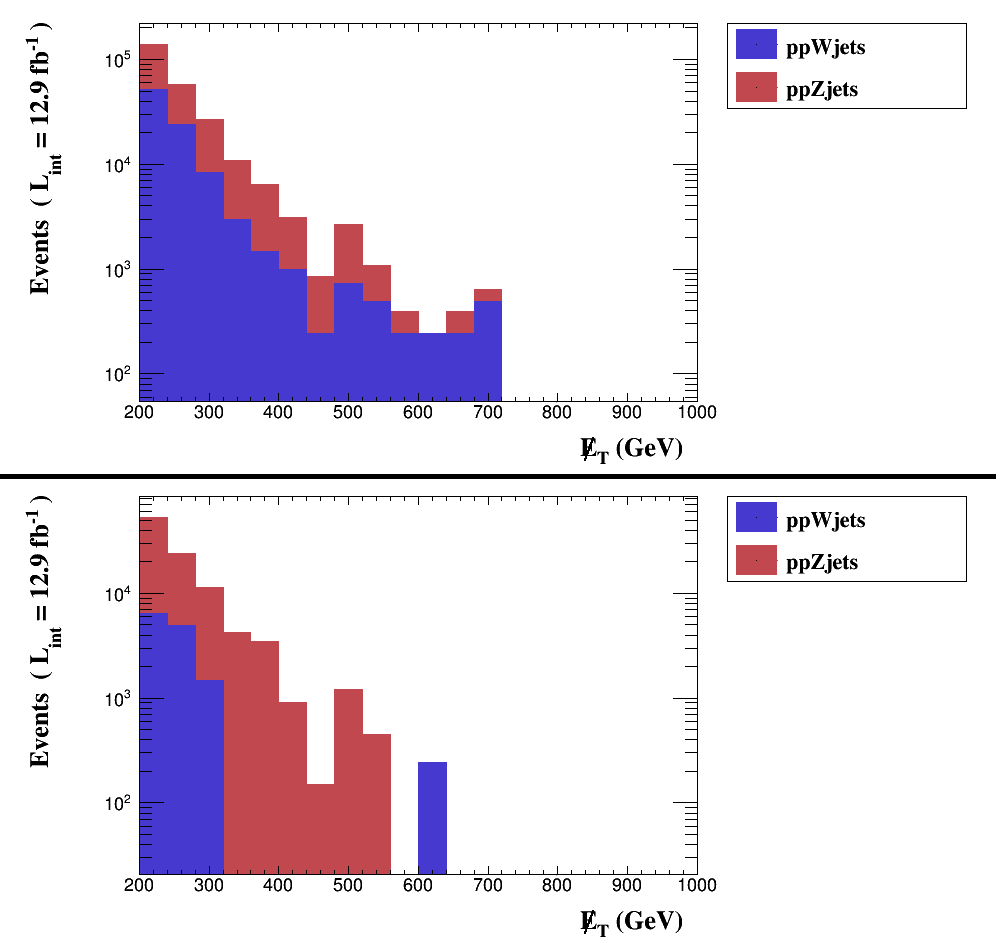
\includegraphics[width=\textwidth]{./sec15/combined_selection.png}
\caption{Histograms showing the number of weighted events against missing transverse energy for the background processes $pp \rightarrow W$ + jets and $\rightarrow Z$ + jets. The upper panel shows the events before any cuts, and the lower panel shows the events after several cuts: jet $p_{\mathrm{T}} > 100$ GeV, $\etmiss > 200$ GeV, $|\eta| < 2.5$, no $b$-quarks, and no leptons.}
\end{figure}

Whilst these results look better, the problems are that the weights are \emph{still} quite high and need to be $\mathcal{O}(1)$ , and that high MET (\etmiss) events are still under-populated even after running lots of \madgraph events (a problem with the law of large numbers -- we need to simulate a \textbf{large number} of events). So to help fix the latter issue, I will try running \madgraph with the same processes but including jet HT (\HT, the scalar sum of transverse momentum) cuts in 200 GeV intervals to produce these high MET events. So I need to produce sets of results with jet HTs of 200--400, 400--600, 600--800, and 800+ (GeV). In the \madgraph input file, I'll need to use the command \verb! set htjmax <value>! to get a minimum HT (default is 0), and \verb!set htjmax <value>! for a maximum HT (default is $-1.0$, meaning no maximum). And the syntax to plot/make cuts on HT in the \madanalysis input file is \verb!THT!. I can also check the list of variables/observables in \textbf{$<$MadAnalysis directory$>$/madanalysis/observable/observable\_list.py}.

These results will need to be handled independently from the other processes (with different HT cuts). I'll need to document the cross sections and weights so I know how I need to include/combine everything. I'm using HT cuts rather than straight MET cuts in the \madgraph input files because HT is an easier variable to deal with than MET. When analysing output from implementing MET cuts -- instead of HT -- with the same ranges, the results were weird and overlapped when they shouldn't have.

So this is the procedure as a more compact list:

\begin{easylist}[enumerate]
& Copy the \madgraph output files (\textbf{tag\_1\_pythia\_events.hep.gz}) from \textbf{/storage/eb16003/submit\_mg/results/} to my \madanalysis directory -- renaming them to something more appropriate -- and consolidate them in the directory \textbf{/storage/eb16003/MadAnalysis/MA5\_v1\_4/Input/}.
& Write an input file for \madanalysis to analyse the .hep.gz files, using Listing \ref{listing:dmmonojinput} as a template. Pay attention to the files I'm importing, the cuts, and the histograms I want plotted. The cuts described in that file are applicable to this analysis because I'm still modelling the backgrounds from the dark matter search in \cite{CMS:2016pod}.
& Make sure I've sourced my \textbf{cms.sh} script to set up the necessary environments.
& Run \madanalysis (with the \verb!-s -R! commands to ensure the creation of the .root file) with the input file.
& Open the PDF in \textbf{/MA5\_v1\_4/$<$name of output directory$>$/PDF/main.pdf} to get information about the weight assigned to the events in each process, the histograms, and the cut flow. I can't open it on Soolin, so just \verb!scp! it to my local machine and use Adobe Reader.
& My macros won't work on the version of ROOT I have on Soolin for whatever reason, so \verb!scp! the \textbf{TheMouth.root} files to my local machine (renaming them to something appropriate to avoid confusion). Then modify my local copies of \textbf{MouthGlobal.h} (see Listing \ref{listing:mouthglobalv1}) in \textbf{/Users/eb16003/PhD\_Software/MadAnalysis/MA5\_v1\_4/Macros\_TheMouth/} to point to the directory containing the renamed \textbf{TheMouth.root} file of the process I want to look at, change the variable \verb!weight! to the value given in the PDF, and make sure \verb!N_BINS!, \verb!X_MIN! and \verb!X_MAX! are the correct values for what I'm looking at.
& Run \textbf{execMouth.C} to print the \emph{weighted} events in each MET bin for the \textbf{TheMouth.root} file I want to look at. Then document the results in a .txt file or an Excel spreadsheet.
% CAN ADD THESE TO THE EXISTING BACKGROUNDS I'VE GOT OR COMPARE THEM WITH THE PAPER.
\end{easylist}

The results from running \madgraph and \madanalysis with different HT ranges (as discussed in the previous paragraphs) are presented below, along with an input file -- created by my \textbf{writeinputfiles\_mg.py} script -- as an example. These runs were implemented with 50,000 events and constrained HT.

One of the \madgraph input files:

\lstinputlisting[language=sh, caption={A \madgraph input file for the SM background process $pp \rightarrow W +$ jets with constrains of jet \HT. File name: ppWjetsHT200-400\_1.input.}]{./sec15/ppWjetsHT200-400_1.input}

The \madanalysis input file to analyse my output from \madgraph:

\lstinputlisting[language=sh, caption={The \madanalysis input file to analyse my SM background processes with constrained \HT. File name: bkgtestHTall.input (v1).}]{./sec15/bkgtestHTallv1.input}

The histograms from \madanalysis showing the number of events vs. total hadronic \HT (THT in \madanalysis syntax):

\begin{figure}[H]
\centering
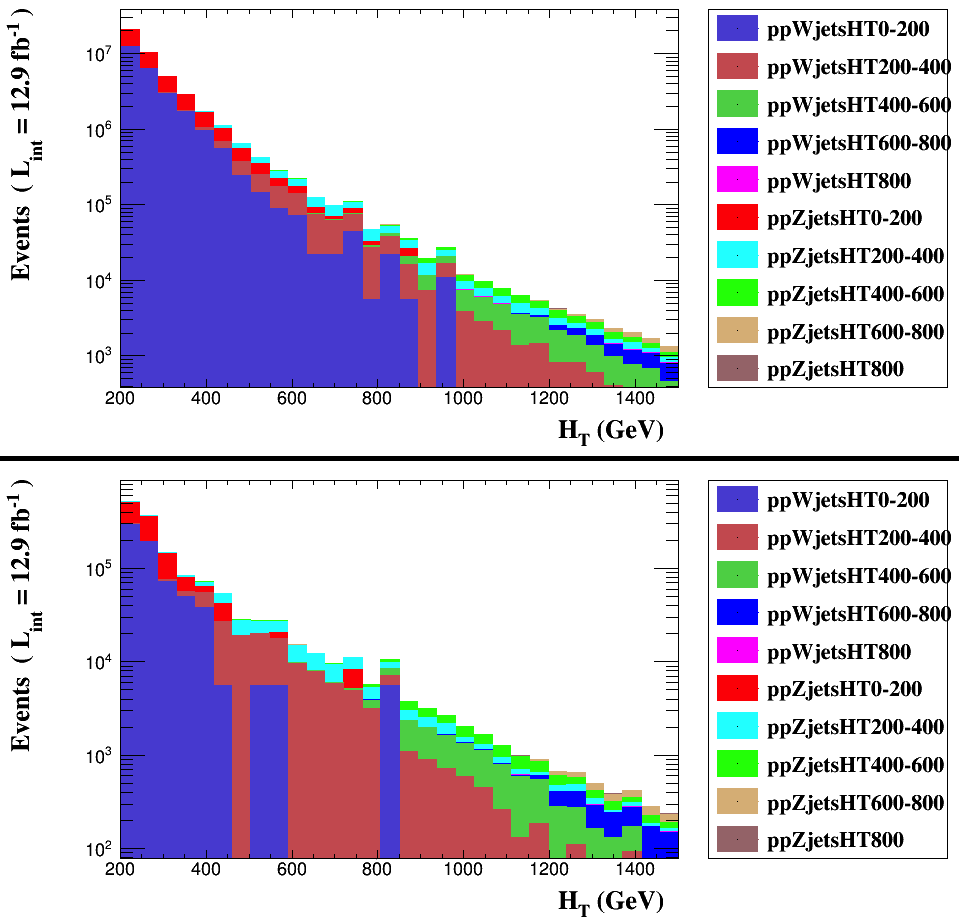
\includegraphics[width=\textwidth]{./sec15/HT_HTranges.png}
\caption{The number of weighted events vs. total hadronic \HT for the Standard Model background processes $pp \rightarrow W +$ jets and $Z +$ jets. These were generated by Monte Carlo with different ranges of \HT. The upper panel shows the events before any cuts, and the lower panel shows the events after several cuts: jet $p_{\mathrm{T}} > 100$ GeV, $\etmiss > 200$ GeV, $|\eta| < 2.5$, no $b$-quarks, and no leptons.}
\end{figure}

The histograms from \madanalysis showing the number of events vs. \etmiss:

\begin{figure}[H]
\centering
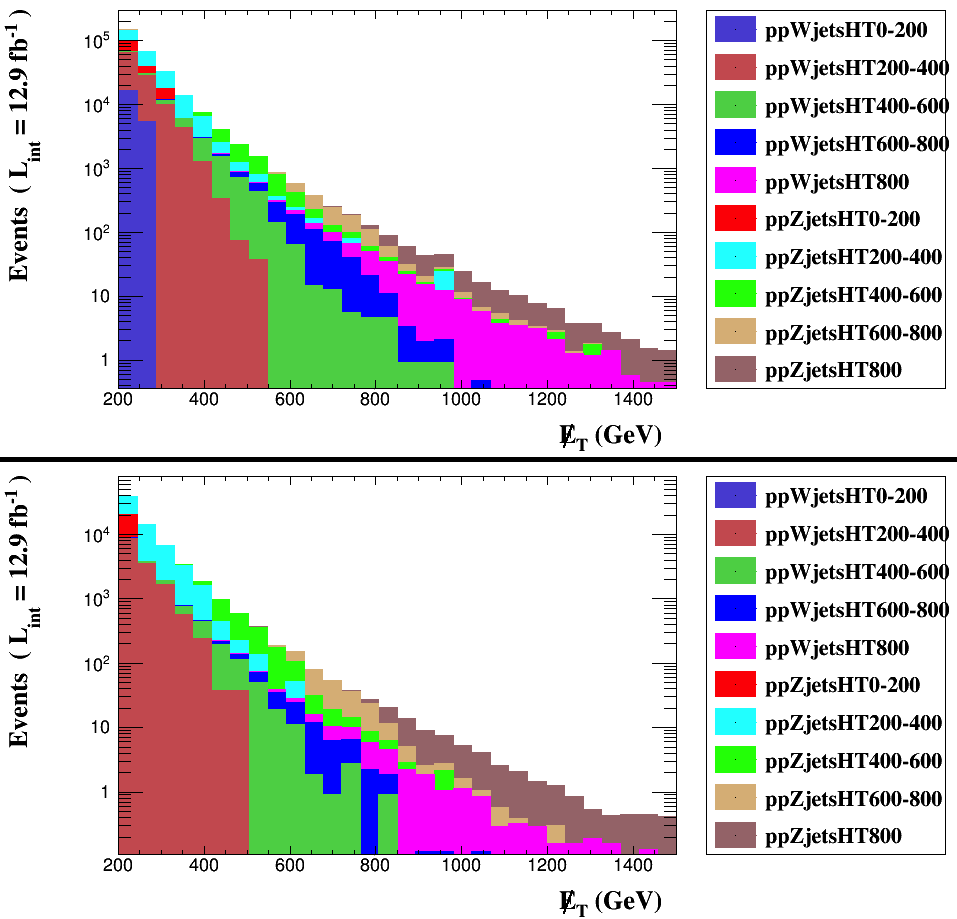
\includegraphics[width=160mm]{./sec15/MET_HTranges.png}
\caption{The number of weighted events vs. \etmiss for the Standard Model background processes $pp \rightarrow W +$ jets and $Z +$ jets. These were generated by Monte Carlo with different ranges of \HT. The upper panel shows the events before any cuts, and the lower panel shows the events after several cuts: jet $p_{\mathrm{T}} > 100$ GeV, $\etmiss > 200$ GeV, $|\eta| < 2.5$, no $b$-quarks, and no leptons.}
\end{figure}

Some numerical data are displayed in the tables below.

$pp \rightarrow W +$ jets:

\begin{table}[H]
\centering
    \begin{tabular}{|l|l|l|l|}
    \hline
    \HT range (GeV) & Generated events & Cross section (pb) & Weight ($\mathcal{L} = 12.9$ fb$^{-1}$) \\ \hline
    $0-200$    & 50,000           & 21381              & 5516                     \\
    $200-400$  & 50,000           & 72.2               & 18                       \\
    $400-600$ & 50,000           & 3.57               & 0.92                     \\
    $600-800$  & 50,000           & 0.461              & 0.12                     \\
    800+     & 50,000           & 0.124              & 0.032                    \\ \hline
    \end{tabular}
\caption{Information from the SM background process $pp \rightarrow W +$ jets, generated by Monte Carlo with different \HT ranges.}
\end{table}

$pp \rightarrow Z +$ jets:

\begin{table}[H]
\centering
    \begin{tabular}{|l|l|l|l|}
    \hline
    \HT range (GeV) & Generated events & Cross section (pb) & Weight ($\mathcal{L} = 12.9$ fb$^{-1}$) \\ \hline
    $0-200$    & 50,000           & 11612              & 2995                     \\
    $200-400$  & 50,000           & 46.5               & 12                       \\
    $400-600$ & 50,000           & 2.24               & 0.58                     \\
    $600-800$  & 50,000           & 0.279              & 0.072                    \\
    800+     & 50,000           & 0.072              & 0.019                    \\ \hline
    \end{tabular}
\caption{Information from the SM background process $pp \rightarrow Z +$ jets, generated by Monte Carlo with different \HT ranges.}
\end{table}

I will be analysing these backgrounds in more detail (with more events) in the future. This subsection can be thought of as a guide and instructions on how to generate and analyse the Monte Carlo data, rather than a complete, comprehensive analysis in and of itself.

Final addition: a script to copy the output files from \madgraph to a destination (so that I don't have to manually copy everything) is displayed below.

\lstinputlisting[language=Python, caption={A script to copy files from a source to a destination. File name: copyfiles.py (v1).}]{./sec15/copyfilesv1.py}
